\documentclass{style/llncs}
% generated by Madoko, version 1.0.3
%mdk-data-line={1}


\usepackage[heading-base={2},section-num={False},bib-label={True}]{madoko2}
%mdk-data-line={19}

  \def\refname{REFERENCES}
%mdk-data-line={1;style/lncs.mdk:6}

    \pagestyle{plain}
\begin{document}



%mdk-data-line={23}
\mdxtitleblockstart{}
%mdk-data-line={23}
\mdxtitle{\mdline{23}A SENSITIVITY ANALYSIS OF A HOSPITAL IN CASE OF FIRE}%mdk
\mdxauthorstart{}
%mdk-data-line={28}
\mdxauthorname{\mdline{28}Anass Rahouti}%mdk

%mdk-data-line={31}
\mdxauthoraddress{\mdline{31}Department of Civil Engineering and Structural Mechanics, Faculty of Engineering, University of Mons}%mdk

%mdk-data-line={34}
\mdxauthoremail{\mdline{34}anass.rahouti@umons.ac.be}%mdk
\mdxauthorend\mdxauthorstart{}
%mdk-data-line={39}
\mdxauthorname{\mdline{39}Selim Datoussaïd}%mdk

%mdk-data-line={42}
\mdxauthoraddress{\mdline{42}Department of Civil Engineering and Structural Mechanics, Faculty of Engineering, University of Mons}%mdk
\mdxauthorend\mdxauthorstart{}
%mdk-data-line={47}
\mdxauthorname{\mdline{47}Ruggiero Lovreglio}%mdk

%mdk-data-line={50}
\mdxauthoraddress{\mdline{50}Department of Civil and Environmental Engineering, University of Auckland}%mdk
\mdxauthorend\mdtitleauthorrunning{}{}\mdxtitleblockend%mdk

%mdk-data-line={25}
\begin{abstract}%mdk

%mdk-data-line={26}
\noindent\mdline{26}One of the primary objectives of fire safety is to guarantee the
evacuation of all the occupants from a building safely. Although fire
safety rules and regulations exist, they remain insufficient to guarantee
the safety of all building occupants and do not prevent the dramatic
events to be repeated. Especially in health care facilities, e.g.
hospitals, care homes, etc., the evacuation procedure is more complex
than in an ordinary building. This is due to multiple reasons such as the
large number of patients requiring assistance to evacuate or the time
required to prepare patients for assisted evacuation. Traditionally,
hospitals focused on horizontal evacuation. Patients should initially be
moved from areas of risk to safe areas. Furthermore, staff to occupant
ratio may be low, especially at night, limiting the ability to instigate
a rapid staff response and evacuation of occupants.%mdk

%mdk-data-line={40}
\mdline{40}Considering the limited number of studies on assisted evacuations, this
work aims to provide a deeper insight on the modeling issues to simulate
such an event. Based upon a preliminary risk analysis using the Fire Risk
Assessment Method for Engineering (FRAME), the most critical floor will
be selected and modeled using Pathfinder, an agent-based evacuation
model. Furthermore, the impact of different percentage of People with
Reduced Mobility will be investigated. Moreover, since the number of
staff may significantly vary in the same scenarios (e.g. during the
night), different ratios of staff to occupant\mdline{48}'\mdline{48}s will be studied to show
the impact of this parameter on the evacuation process.%mdk

%mdk-data-line={51}
\mdline{51}\emph{Keywords}\mdline{51}: Evacuation Modeling, Assisted Evacuation, Fire Safety, Hospital, FRAME%mdk
%mdk
\end{abstract}%mdk

%mdk-data-line={54}
\section{\mdline{54}1.\hspace*{0.5em}\mdline{54}INTRODUCTION}\label{sec-introduction}%mdk%mdk

%mdk-data-line={56}
\noindent\mdline{56}Each year, in Belgium, fire kills and costs money. In fact, in 2013,
Belgian fire and rescue services attended over 22.733 fires including 236
in care homes and 79 in hospitals\mdline{58}~[\mdcite{1}{27}]\mdline{58}. These fires killed 51
people and injured over 1189\mdline{59}~[\mdcite{1}{27}]\mdline{59}. In health care facilities,
patients may start fires, either accidentally or deliberately,
particularly by those who are elderly, have learning difficulties, or are
young people with disabilities. Those who suffer from mental illness may
be particularly prone to starting fires. In these particular buildings,
the occupants will be a mixture of patients, staff and visitors. Staff
can reasonably be expected to have an understanding of the layout of the
premises (or of the part in which they work), while visitors are unlikely
to have knowledge of alternative escape routes. Patients may have limited
knowledge, but will generally be guided or assisted to a place of safety
by staff or visitors. Further to this, health care facilities present a
set of challenges from the perspective of fire safety. This is due to
multiple reasons such as the large number of patients requiring
assistance to evacuate or the time required to prepare patients for
assisted evacuation. Furthermore, staff to occupant\mdline{73}'\mdline{73}s ratio may be low,
especially at night, limiting the ability to instigate a rapid staff
response and evacuation of occupants.%mdk

%mdk-data-line={77}
\mdline{77}How quickly people can evacuate will depend on their level of reliance on
staff and it will therefore be helpful to consider the various categories
of patient dependencies: \mdline{79}\textbf{Independent}\mdline{79} (ambulant), the mobility of
patients is not impaired in any way and they are able to physically leave
the premises without the assistance of staff or, if they experience some
mobility impairment, they are able to leave with minimal assistance from
another person; \mdline{83}\textbf{Dependent}\mdline{83} (non-ambulant), all patients except those
defined as independent or very high dependency. This category also
includes children and mental health patients regardless of their
independent mobility; \mdline{86}\textbf{Very high dependency}\mdline{86} (non-ambulant), those
patients whose clinical treatment and/or condition create a high
dependency on staff. This includes those in intensive care/intensive
therapy units and operating rooms and those where evacuation would prove
potentially life threatening. Patients being cared for in health care
premises will vary considerably in terms of mobility and levels of
awareness during a fire situation. There may be patients who exhibit
severe mobility restriction but will have a good awareness of the
situation, being able to co-operate with staff. Others may exhibit normal
mobility, but their level of awareness may be such that they present
unpredictable behavior (including violent behavior), which may impede
staff in an emergency.%mdk

%mdk-data-line={99}
\mdline{99}It is true that the ideal way to determine the egress time required and the best evacuation 
 strategy would be to conduct some timed evacuation drills involving the movement of all the patients. However, conducting
 real experiments in health care environments is prohibited
since such experiments will be really hazardous in presence of vulnerable
people. Another alternative consists on using simulation tools. This would identify many simple problems that may be rectified before any emergency evacuation should occur. 
 In fact, it is well known that evacuation models are powerful tools to study the
evacuation process in different scenarios and
applications\mdline{106}~[\mdcite{3}{1}, \mdcite{4}{4}, \mdcite{5}{7}, \mdcite{2}{15}, \mdcite{6}{19}]\mdline{106}. We can find several reviews\mdline{106}~[\mdcite{3}{1}, \mdcite{2}{15}]\mdline{106} that
show the capabilities and limitations of these types of models. These
reviews show that, apart from their possibilities, it is difficult to
apply directly the current evacuation models to the scenarios that
involve assisted evacuations, due to the presence of vulnerable people
who cannot evacuate by themselves (health care facilities, kindergartens
and schools). However, few of them are able to simulate assisted
evacuations. For example, the EXITT\mdline{113}~[\mdcite{7}{22}]\mdline{113} model includes two types of
occupants, the able-bodied people and the people with reduced mobility
(PRM) in need of assistance to evacuate the building. Decision rules
apply only to the first type, and the latter type follows the decisions
and movements of their attendants. The BUMMPEE\mdline{117}~[\mdcite{8}{5}]\mdline{117} model can simulate the
evacuation of people with disabilities, and their interaction with the
built environment. However, it is not clear whether this model can
simulate assisted evacuations. The buildingEXODUS\mdline{120}~[\mdcite{9}{21}]\mdline{120} model includes a
theoretical model comprising algorithms derived to represent the use of
patient transportation devices during the evacuation process\mdline{122}~[\mdcite{10}{17}]\mdline{122}. In
addition, there are two models that specialize in the evacuation of
hospitals: The G-HES (Glasgow Hospital Evacuation Simulator)\mdline{124}~[\mdcite{11}{18}]\mdline{124} and the
Assisted Evacuation Simulation System\mdline{125}~[\mdcite{12}{36}]\mdline{125}. Both models have been
developed to consider assisted evacuations. However, they are not
publicly available\mdline{127}~[\mdcite{13}{3}]\mdline{127}.%mdk

%mdk-data-line={129}
\mdline{129}Another alternative is the use of other existing evacuation (or general)
models that are not explicitly designed to simulate assisted evacuations
but they can be flexible enough to archive this goal (e.g.
Pathfinder\mdline{132}~[\mdcite{14}{35}]\mdline{132}, FDS+Evac\mdline{132}~[\mdcite{15}{23}]\mdline{132}, STEPS\mdline{132}~[\mdcite{16}{12}]\mdline{132}, etc.). In fact, some of them
allow the simulation of additional behaviors, such as travel itineraries
assigned to occupants, delays, etc. This could be used to simulate
prescript assisted evacuation procedures.%mdk

%mdk-data-line={137}
\mdline{137}Only a limited number of studies have examined the assisted evacuations
using the general models. One of the studies to do so was completed by
Golmohammadi and Shimshak\mdline{139}~[\mdcite{17}{28}]\mdline{139} showed an analytical approximation to
analyze the horizontal and the vertical evacuation times, considering
three types of patients. This analytical model permits the user to
consider the number and the category of patients and the number of the
staff members and the availability of the elevators. Alonso\mdline{143}~[\mdcite{18}{2}]\mdline{143}
performed an interesting study using STEPS model. She simulated the
impact of staff to occupant\mdline{145}'\mdline{145}s ratio on the relocation process of patients
on a sleeping room floor in a health care facility. She highlighted the
lack of empirical data and the limitations of using a general model for
this kind of scenarios, and suggested future development for addressing
the problem of simulating assisted evacuations. Ursetta et al.\mdline{149}~[\mdcite{19}{26}]\mdline{149}
simulated the evacuation process of an Italian hospital ward in case of
fire using Pathfinder.%mdk

%mdk-data-line={153}
\mdline{153}Despite that the modeling of assisted evacuations is restricted, it is
commonly agreed that it is needed to differentiate between self-reliant
(ambulant) and incapacitated (non-ambulant) patients. Moreover, all the
incapacitated patients have a preparation time that may depend on the
type of their disability. For some patients, this preparation time will
include the processes to stabilize the patient\mdline{158}'\mdline{158}s condition (e.g.
operating room), to disconnect the patients from equipment, to move a
patient from the bed to a transportation device (e.g. Evac+Chair,
stretcher, etc.), to just help them to get dressed or to gather their
belongings. Currently, there is a lack of data related to these
preparation times and transportation speeds. The values of these
parameters are limited. For example, Adams and Galea\mdline{164}~[\mdcite{20}{10}]\mdline{164} present an
experimental study to evaluate the performance of the movement devices
used to assist PRM in high-rise building evacuations. Based on this
experimental study, Hunt, Galea and Lawrence\mdline{167}~[\mdcite{21}{20}]\mdline{167} conducted a numerical
study to analyze the performance of trained hospital staff using movement
assist devices to evacuate PRM. Other studies\mdline{169}~[\mdcite{22}{9}, \mdcite{23}{25}]\mdline{169} show some possible
ranges and values for preparation times considering different types of
patients for the sleeping areas.%mdk

%mdk-data-line={173}
\mdline{173}The study undertaken here aimed (1) to simulate prescript assisted
evacuation using Pathfinder; (2) to evaluate the impact of different
percentages of people with reduced mobility on the evacuation process,
especially on the Required Safe Egress Time (RSET) – the time required by
the occupants to leave the floor and escape to a place of reasonable
safety; and, since the number of staff may significantly vary in the same
scenarios (e.g. during the night), to study the effect of staff to
patient\mdline{180}'\mdline{180}s ratio on the evacuation process.%mdk

%mdk-data-line={182}
\section{\mdline{182}2.\hspace*{0.5em}\mdline{182}METHODS}\label{sec-methods}%mdk%mdk

%mdk-data-line={184}
\noindent\mdline{184}The methods employed in this study combine risk assessment
and evacuation modeling techniques. The initial phase of the study was
therefore the use of the Fire Risk Assessment Method for Engineering\mdline{186}~[\mdcite{25}{30}]\mdline{186}
to identify the most critical floor. The layout of this floor was modeled
within Pathfinder using a third-party (PyroSim). And finally, a number of
patients with different individual characteristics were created and
distributed throughout the model.%mdk

%mdk-data-line={192}
\mdline{192}When possible, the input of the evacuation model was calibrated using
experimental data rather than the default settings of the model. This had
the effect of making the evacuation scenarios as realistic as possible.%mdk

%mdk-data-line={196}
\subsection{\mdline{196}2.1.\hspace*{0.5em}\mdline{196}FIRE RISK ASSESSMENT METHOD FOR ENGINEERING}\label{sec-fire-risk-assessment-method-for-engineering}%mdk%mdk

%mdk-data-line={198}
\noindent\mdline{198}The Fire Risk Assessment Method for Engineering developed by De
Smet\mdline{199}~[\mdcite{25}{30}]\mdline{199}, is a comprehensive, transparent and practical calculation
method for fire risks in buildings. It is a tool to help a fire
protection engineer to define a sufficient and cost effective fire safety
concept for new or existing buildings. The FRAME method calculates the
fire risk in buildings for the property and the content, for the
occupants and for the activities in it. The method is not suitable for
open-air environment.%mdk

%mdk-data-line={207}
\mdline{207}Apart from its use in airports\mdline{207}~[\mdcite{26}{31}]\mdline{207}, industry\mdline{207}~[\mdcite{27}{32}]\mdline{207} and cultural
heritage buildings\mdline{208}~[\mdcite{29}{8}, \mdcite{28}{33}]\mdline{208} this method has been employed mainly for
health care facilities\mdline{209}~[\mdcite{31}{6}, \mdcite{30}{34}]\mdline{209}.%mdk

%mdk-data-line={211}
\subsection{\mdline{211}2.2.\hspace*{0.5em}\mdline{211}PATHFINDER}\label{sec-pathfinder}%mdk%mdk

%mdk-data-line={213}
\noindent\mdline{213}Pathfinder is an agent-based egress and human movement simulator. It is
developed by Thunderhead Engineering. Its purpose is to provide an
analytical evacuation tool that could be coupled with an external fire
model such as FDS (Fire Dynamics Simulator)\mdline{216}~[\mdcite{32}{16}]\mdline{216} to form portion of
hazard analysis. The occupants are represented as circles moving in a
continuous space. It uses two different ways to model the evacuation
process (1) and agent-based model (steering) or (2) based on the method
of Mowrer ad Nelson (flow model)\mdline{220}~[\mdcite{33}{24}]\mdline{220}. The model considers individual
profiles (walking speed and pre-movement times) implemented through
distribution laws.%mdk

%mdk-data-line={224}
\section{\mdline{224}3.\hspace*{0.5em}\mdline{224}MODEL CASE STUDY}\label{sec-model-case-study}%mdk%mdk

%mdk-data-line={226}
\subsection{\mdline{226}3.1.\hspace*{0.5em}\mdline{226}FLOOR LAYOUT}\label{sec-floor-layout}%mdk%mdk

%mdk-data-line={228}
\noindent\mdline{228}The layout of the modeled floor is shown in Figure\mdline{228}~\mdref{fig-layout}{\mdcaptionlabel{1}}\mdline{228}. As
shown in this Figure, this floor contains 42 rooms: 14 single rooms (from
13 to 26) and 28 double rooms (the others). This floor had three exits
associated to the emergency staircases, two nurses\mdline{231}'\mdline{231} stations and some
technical rooms. The lifts are not used during the evacuation process.
The fire is supposed located in room 13. Therefore, the East Exit is
supposed non-functional during the evacuation processes simulated.%mdk

%mdk-data-line={236}
\begin{figure}[tbp]%mdk
\begin{mdcenter}%mdk

%mdk-data-line={237}
\noindent\mdline{237}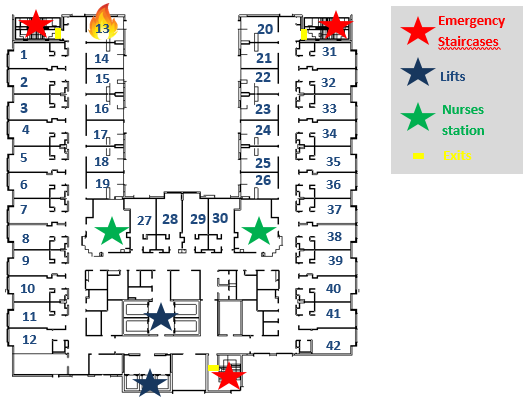
\includegraphics[keepaspectratio=true,width=\dimmin{}{\dimwidth{0.90}}]{images/FIG_1}{}\mdline{237}%mdk

%mdk-data-line={238}
\mdhr{}%mdk

%mdk-data-line={239}
\noindent\mdline{239}\mdcaption{\textbf{Figure~\mdcaptionlabel{1}.}~\mdcaptiontext{Layout of the 6th floor of the G bloc of the Clinique Sainte Elisabeth}}%mdk
%mdk
\end{mdcenter}\label{fig-layout}%mdk
%mdk
\end{figure}%mdk

%mdk-data-line={241}
\subsection{\mdline{241}3.2.\hspace*{0.5em}\mdline{241}PROFILE OF THE OCCUPANTS}\label{sec-profile-of-the-occupants}%mdk%mdk

%mdk-data-line={243}
\noindent\mdline{243}For the simulations, we considered two types of patients: ambulant
patients and non-ambulant patients.%mdk

%mdk-data-line={246}
\mdline{246}For ambulant patients, the movement and behavior of each individual is
described by several parameters such as the pre-evacuation time and the
horizontal walking speed.%mdk

%mdk-data-line={250}
\mdline{250}For non-ambulant patients, the movement and behavior of each patient is
described by several parameters such as the pre-movement time, which is
divided into two components: the waiting time – the time undertaken by
the member(s) of staff to reach the room of the patient – and the
preparation time – the time undertaken by the member(s) of the staff to
move the patient to a wheelchair or to another transportation device.
Another parameter is the transportation walking speed – the walking speed
of the member(s) of the staff while transporting the patient to another
place of safety or while walking with the patients.%mdk

%mdk-data-line={260}
\mdline{260}The values used for the simulations are shown in the
Tables\mdline{261}~\mdref{tab-pre-evac}{\mdcaptionlabel{1}}\mdline{261} and\mdline{261}~\mdref{tab-prep-trans}{\mdcaptionlabel{2}}\mdline{261}. The waiting times are
dependent on the scenario simulated. So, they are not explicitly
described here.%mdk

%mdk-data-line={265}
\begin{table}[tbp]%mdk
\begin{mdcenter}%mdk
\begin{mdtabular}{4}{\dimeval{(\linewidth)/4}}{1ex}%mdk
\begin{tabular}{cccc}\cmidrule{2-2}\cmidrule{3-3}\cmidrule{4-4}
{\bfseries\mdline{267}}&{\bfseries\mdline{267} Mean}&{\bfseries\mdline{267} St. Dev.}&{\bfseries\mdline{267} Range}\\

\midrule
\mdline{269} Pre-evacuation time (s)\mdline{269}~[\mdcite{35}{13}, \mdcite{34}{14}]&\mdline{269} 50.8&\mdline{269} \mdline{269}-&\mdline{269} 30 – 66\\
\mdline{270} Horizontal walking speed (m/s)\mdline{270}~[\mdcite{36}{29}]\mdline{270}&\mdline{270} 1.00&\mdline{270} 0.42&\mdline{270} 0.10 – 1.77\\
\end{tabular}\end{mdtabular}

%mdk-data-line={273}
\mdhr{}%mdk

%mdk-data-line={274}
\noindent\mdline{274}\mdcaption{\textbf{Table~\mdcaptionlabel{1}.}~\mdcaptiontext{Pre-evacuation time and horizontal walking speed for ambulant patients.}}%mdk
%mdk
\end{mdcenter}\label{tab-pre-evac}%mdk
%mdk
\end{table}%mdk

%mdk-data-line={275}
\begin{table}[tbp]%mdk
\begin{mdcenter}%mdk
\begin{mdtabular}{6}{\dimeval{(\linewidth)/6}}{1ex}%mdk
\begin{tabular}{cllccc}\cmidrule{2-2}\cmidrule{3-3}\cmidrule{4-4}
\multicolumn{3}{c}{{\bfseries\mdline{277}}}&\multicolumn{1}{c}{{\bfseries\mdline{277} Mean}}&\multicolumn{1}{c}{{\bfseries\mdline{277}St. Dev.}}&{\bfseries\mdline{277}Range}\\

\midrule
\mdline{279} Dependent patients\mdline{279}~[\mdcite{10}{17}]\mdline{279}&\mdline{279} Evacuation&\mdline{279} Preparation time (s)&\mdline{279} 32.7&\mdline{279} 5.3&\mdline{279} \mdline{279}-\\
\cmidrule{3-3}\cmidrule{4-4}\cmidrule{5-5}\cmidrule{6-6}
\mdline{281}&\mdline{281}&\mdline{281} Transportation walking speed (m/s)&\mdline{281} 1.46&\mdline{281} 0.09&\mdline{281} \mdline{281}-\\
\cmidrule{2-2}\cmidrule{3-3}\cmidrule{4-4}\cmidrule{5-5}\cmidrule{6-6}
\mdline{283}&\mdline{283} Carry&\mdline{283} Preparation time (s)&\mdline{283} 41.5&\mdline{283} 7.9&\mdline{283}\\
\cmidrule{3-3}\cmidrule{4-4}\cmidrule{5-5}\cmidrule{6-6}
\mdline{285}&\mdline{285}&\mdline{285} Transportation walking speed (m/s)&\mdline{285} 1.50&\mdline{285} 0.10&\mdline{285} \mdline{285}-\\
\cmidrule{2-2}\cmidrule{3-3}\cmidrule{4-4}\cmidrule{5-5}\cmidrule{6-6}
\mdline{287}&\mdline{287} Stretcher&\mdline{287} Preparation time (s)&\mdline{287} 77.7&\mdline{287} 19.2&\mdline{287} \mdline{287}-\\
\cmidrule{3-3}\cmidrule{4-4}\cmidrule{5-5}\cmidrule{6-6}
\mdline{289}&\mdline{289}&\mdline{289} Transportation walking speed (m/s)&\mdline{289} 1.04&\mdline{289} 0.09&\mdline{289} \mdline{289}-\\
\cmidrule{2-2}\cmidrule{3-3}\cmidrule{4-4}\cmidrule{5-5}\cmidrule{6-6}
\mdline{291}&\mdline{291} Rescue&\mdline{291} Preparation time (s)&\mdline{291} 65.2&\mdline{291} 14.1&\mdline{291} \mdline{291}-\\
\cmidrule{3-3}\cmidrule{4-4}\cmidrule{5-5}\cmidrule{6-6}
\mdline{293}&\mdline{293}&\mdline{293} Transportation walking speed (m/s)&\mdline{293} 0.89&\mdline{293} 0.24&\mdline{293} \mdline{293}-\\
\midrule
\multicolumn{2}{c}{\mdline{295} Highly dependent patients\mdline{295}~[\mdcite{11}{18}]\mdline{295}}&\mdline{295} Preparation time (s)&\multicolumn{1}{c}{\mdline{295} \mdline{295}-}&\mdline{295} \mdline{295}-&\mdline{295} 180-900\\
\cmidrule{2-2}\cmidrule{3-3}\cmidrule{4-4}\cmidrule{5-5}
\multicolumn{2}{c}{\mdline{297}}&\mdline{297} Transportation walking speed (m/s)&\multicolumn{1}{c}{\mdline{297} 0.40}&\mdline{297} 0.04&\mdline{297} \mdline{297}-\\
\midrule
\end{tabular}\end{mdtabular}

%mdk-data-line={300}
\mdhr{}%mdk

%mdk-data-line={301}
\noindent\mdline{301}\mdcaption{\textbf{Table~\mdcaptionlabel{2}.}~\mdcaptiontext{Preparation time and transportation walking speed for non-ambulant patients.}}%mdk
%mdk
\end{mdcenter}\label{tab-prep-trans}%mdk
%mdk
\end{table}%mdk

%mdk-data-line={302}
\mdline{302}There is a lack of data regarding the number of attendants needed to
evacuate non-ambulant patients. Table\mdline{303}~\mdref{tab-operators-roles}{\mdcaptionlabel{3}}\mdline{303} shows some
values found on the available literature for dependent patients. As it is
shown in this table, the type of the transportation device used defines
the number of required attendants to prepare the patient and to assist on
the evacuation process. Comparing the different devices, we can conclude
that evacuation chair and the rescue sheet require the minimum number of
attendants (two).%mdk

%mdk-data-line={311}
\mdline{311}For highly dependent patients, the number of attendants needed is
unknown. Therefore, we suppose that two attendants are enough.%mdk

%mdk-data-line={314}
\begin{table}[tbp]%mdk
\begin{mdcenter}%mdk
\begin{mdtabular}{7}{\dimeval{(\linewidth)/7}}{1ex}%mdk
\begin{tabular}{ccccccc}{\bfseries\mdline{316} Experiment}&{\bfseries\mdline{316} Role}&{\bfseries\mdline{316} Stretcher}&{\bfseries\mdline{316} Evacuation}&{\bfseries\mdline{316} Carry Chair}&{\bfseries\mdline{316} Carry Chair}&{\bfseries\mdline{316} Rescue}\\
{\bfseries\mdline{317} Phase}&{\bfseries\mdline{317}}&{\bfseries\mdline{317}}&{\bfseries\mdline{317} Chair}&{\bfseries\mdline{317} (Male team)}&{\bfseries\mdline{317} (Female team)}&{\bfseries\mdline{317} Sheet}\\

\midrule
\mdline{319} Preparation&\mdline{319} Essential&\mdline{319} 2&\mdline{319} 2&\mdline{319} 2&\mdline{319} 2&\mdline{319} 2\\
\cmidrule{2-2}\cmidrule{3-3}\cmidrule{4-4}\cmidrule{5-5}\cmidrule{6-6}\cmidrule{7-7}
\mdline{321}&\mdline{321} Major&\mdline{321} 1&\mdline{321} 0&\mdline{321} 1&\mdline{321} 1&\mdline{321} 0\\
\cmidrule{2-2}\cmidrule{3-3}\cmidrule{4-4}\cmidrule{5-5}\cmidrule{6-6}\cmidrule{7-7}
\mdline{323}&\mdline{323} Minor&\mdline{323} 1&\mdline{323} 0&\mdline{323} 0&\mdline{323} 1&\mdline{323} 0\\
\midrule
\mdline{325} Corridor&\mdline{325} Essential&\mdline{325} 4&\mdline{325} 1&\mdline{325} 1&\mdline{325} 1&\mdline{325} 2\\
\cmidrule{2-2}\cmidrule{3-3}\cmidrule{4-4}\cmidrule{5-5}\cmidrule{6-6}\cmidrule{7-7}
\mdline{327}&\mdline{327} Major&\mdline{327} 0&\mdline{327} 1&\mdline{327} 1&\mdline{327} 1&\mdline{327} 0\\
\cmidrule{2-2}\cmidrule{3-3}\cmidrule{4-4}\cmidrule{5-5}\cmidrule{6-6}\cmidrule{7-7}
\mdline{329}&\mdline{329} Minor&\mdline{329} 0&\mdline{329} 0&\mdline{329} 1&\mdline{329} 2&\mdline{329} 0\\
\midrule
\multicolumn{2}{c}{\mdline{331} Total number of attendants}&\mdline{331} 4&\mdline{331} 2&\mdline{331} 3&\mdline{331} 4&\mdline{331} 2\\
\midrule
\end{tabular}\end{mdtabular}

%mdk-data-line={334}
\mdhr{}%mdk

%mdk-data-line={335}
\noindent\mdline{335}\mdcaption{\textbf{Table~\mdcaptionlabel{3}.}~\mdcaptiontext{[The number of operators and their roles for each device [\mdcite{10}{17}]]}}%mdk
%mdk
\end{mdcenter}\label{tab-operators-roles}%mdk
%mdk
\end{table}%mdk

%mdk-data-line={336}
\subsection{\mdline{336}3.3.\hspace*{0.5em}\mdline{336}EVACUATION STRATEGY}\label{sec-evacuation-strategy}%mdk%mdk

%mdk-data-line={338}
\noindent\mdline{338}Traditionally, hospitals focused on horizontal evacuation\mdline{338}~[\mdcite{37}{11}]\mdline{338}. Patients
should initially be moved from areas of risk to areas where a
\mdline{340}\textquotedblleft{}shelter-in-place\textquotedblright{}\mdline{340} posture can be maintained; usually in
separate smoke compartments. As long as it is safe to remain in the
\mdline{342}\textquotedblleft{}shelter-in-place\textquotedblright{}\mdline{342} position, it is the preferred choice to
attempting vertical evacuation. Therefore, in this study, we are only
considering horizontal evacuation.%mdk

%mdk-data-line={346}
\subsection{\mdline{346}3.4.\hspace*{0.5em}\mdline{346}EVACUATION PROCEDURE}\label{sec-evacuation-procedure}%mdk%mdk

%mdk-data-line={348}
\noindent\mdline{348}In health care facilities, in case of fire, the objective of the staff is
to evacuate as many patients as possible\mdline{349}~[\mdcite{18}{2}, \mdcite{10}{17}]\mdline{349}. So, in this study,
people in immediate danger are evacuated first, followed by ambulant
patients and then non-ambulant patients. For non-ambulant patients, those
requiring some transport assistance are evacuated first (wheelchair,
evacuation chair), followed by those requiring transport assistance
(rescue sheet) and then patients who are being treated and/or would be
difficult to evacuate (i.e. Operating Room, ICU, obese, dangerous).%mdk

%mdk-data-line={357}
\mdline{357}Furthermore, we considered that attendants use the nearest exit and that
only two exits were available.%mdk

%mdk-data-line={360}
\subsection{\mdline{360}3.5.\hspace*{0.5em}\mdline{360}SCENARIOS MODELED}\label{sec-scenarios-modeled}%mdk%mdk

%mdk-data-line={362}
\noindent\mdline{362}Typically, hospital rooms are single or double occupancy but for the
hypothetical scenarios simulated, all the rooms are considered as single
occupancy. Furthermore, the 42 rooms are considered as fully occupied
(see Figure\mdline{365}~\mdref{path-geom}{\mdcaptionlabel{2}}\mdline{365}).%mdk

%mdk-data-line={367}
\begin{figure}[tbp]%mdk
\begin{mdcenter}%mdk

%mdk-data-line={368}
\noindent\mdline{368}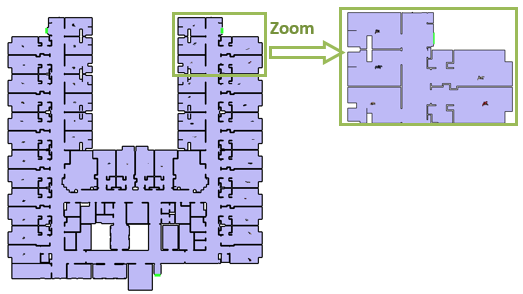
\includegraphics[keepaspectratio=true,width=\dimmin{}{\dimwidth{1.00}}]{images/FIG_2}{}\mdline{368}%mdk

%mdk-data-line={369}
\mdhr{}%mdk

%mdk-data-line={370}
\noindent\mdline{370}\mdcaption{\textbf{Figure~\mdcaptionlabel{2}.}~\mdcaptiontext{Pathfinder geometry shown with sample occupancy}}%mdk
%mdk
\end{mdcenter}\label{path-geom}%mdk
%mdk
\end{figure}%mdk

%mdk-data-line={374}
\subsubsection{\mdline{374}3.5.1.\hspace*{0.5em}\mdline{374}Scenario 1}\label{sec-scenario-1}%mdk%mdk

%mdk-data-line={376}
\noindent\mdline{376}All the patients are considered as ambulant. The other scenarios will be
compared to this basis scenario.%mdk

%mdk-data-line={379}
\subsubsection{\mdline{379}3.5.2.\hspace*{0.5em}\mdline{379}Scenario 2}\label{sec-scenario-2}%mdk%mdk

%mdk-data-line={381}
\noindent\mdline{381}A mix of ambulant and non-ambulant patients was considered with different
percentages of independent, dependent and highly dependent patients. We
considered 6 attendants present to assist on the evacuation of
non-ambulant patients. Therefore, three emergency groups were formed by
two attendants for assisting each patient. The Table\mdline{385}~\mdref{tab-scenario2}{\mdcaptionlabel{4}}\mdline{385} shows the
sub-scenarios simulated.%mdk

%mdk-data-line={388}
\begin{table}[tbp]%mdk
\begin{mdcenter}%mdk
\begin{mdtabular}{4}{\dimeval{(\linewidth)/4}}{1ex}%mdk
\begin{tabular}{cccc}{\bfseries\mdline{390} Sub-scenario}&{\bfseries\mdline{390} Number of independent patients}&{\bfseries\mdline{390} Number of dependent patients}&{\bfseries\mdline{390} Number of highly dependent patients}\\

\midrule
\mdline{392} 2.1&\mdline{392} 28&\mdline{392} 14&\mdline{392} 0\\
\mdline{393} 2.2&\mdline{393} 28&\mdline{393} 7&\mdline{393} 7\\
\midrule
\end{tabular}\end{mdtabular}

%mdk-data-line={395}
\mdhr{}%mdk

%mdk-data-line={396}
\noindent\mdline{396}\mdcaption{\textbf{Table~\mdcaptionlabel{4}.}~\mdcaptiontext{Sub-scenarios simulated for Scenario 2}}%mdk
%mdk
\end{mdcenter}\label{tab-scenario2}%mdk
%mdk
\end{table}%mdk

%mdk-data-line={397}
\subsubsection{\mdline{397}3.5.3.\hspace*{0.5em}\mdline{397}Scenario 3}\label{sec-scenario-3}%mdk%mdk

%mdk-data-line={399}
\noindent\mdline{399}Like Scenario 2, a mix of ambulant and non-ambulant patients is
considered but here the percentage of the patients is constant (1/3
independent, 1/3 dependent and 1/3 highly dependent). In order to
evaluate the effect of different staff to patient\mdline{402}'\mdline{402}s ratios on the
evacuation process, we considered different numbers of attendants
(nurses): 4, 8 and 12. The Table\mdline{404}~\mdref{tab-scenario3}{\mdcaptionlabel{5}}\mdline{404} shows the emergency groups formed for
the different sub-scenarios.%mdk

%mdk-data-line={407}
\begin{table}[tbp]%mdk
\begin{mdcenter}%mdk
\begin{mdtabular}{3}{\dimeval{(\linewidth)/3}}{1ex}%mdk
\begin{tabular}{ccc}{\bfseries\mdline{409} Sub-scenario}&{\bfseries\mdline{409} Number of attendants}&{\bfseries\mdline{409} Emergency groups}\\

\midrule
\mdline{411} 3.1&\mdline{411} 4&\mdline{411} 2\\
\mdline{412} 3.2&\mdline{412} 8&\mdline{412} 4\\
\mdline{413} 3.3&\mdline{413} 12&\mdline{413} 6\\
\midrule
\end{tabular}\end{mdtabular}

%mdk-data-line={415}
\mdhr{}%mdk

%mdk-data-line={416}
\noindent\mdline{416}\mdcaption{\textbf{Table~\mdcaptionlabel{5}.}~\mdcaptiontext{Sub-scenarios simulated for Scenario 3}}%mdk
%mdk
\end{mdcenter}\label{tab-scenario3}%mdk
%mdk
\end{table}%mdk

%mdk-data-line={418}
\section{\mdline{418}4.\hspace*{0.5em}\mdline{418}RESULTS AND DISCUSSION}\label{sec-results-and-discussion}%mdk%mdk

%mdk-data-line={420}
\subsection{\mdline{420}4.1.\hspace*{0.5em}\mdline{420}FRAME METHOD RESULTS}\label{sec-frame-method-results}%mdk%mdk

%mdk-data-line={422}
\noindent\mdline{422}The Table\mdline{422}~\mdref{tab-frame}{\mdcaptionlabel{6}}\mdline{422} presents the results of the Fire Risk Assessment Method for
Engineering performed on the G Bloc of the \mdline{423}\textquotedblleft{}Clinique Sainte Elisabeth\textquotedblright{}\mdline{423},
located at Namur (Belgium). The calculation of the potential risk is
carried on each floor of this building but only for the characteristic
premises of the floor in question. The method gives the following
results: the calculated risk for the property \mdline{427}\&\mdline{427} content (R), the
calculated risk for the occupants (R1) and the calculated risk for the
activities (R2). For a well-protected compartment, the three values shell
be below one.%mdk

%mdk-data-line={432}
\mdline{432}In general, the results of this analysis demonstrate that the building is
well protected (R\mdline{433}\textless{}\mdline{433}1) against fire excluding the technical premise of
the 7th floor in which the potential risk for the occupants is greater
than one. That conclusion is, in fact, expected since the recent
conception of the G Bloc strictly follows the Belgian Prescriptive Codes
(AR 6/11/1997).%mdk

%mdk-data-line={439}
\mdline{439}For the upper floor, the risk for the occupants is important due to the
presence of the machinery of the ventilation and heating. In addition,
its height makes it difficult to access for firefighters. However, this
floor is only accessible for the staff members who are trained to fight
the fire.%mdk

%mdk-data-line={445}
\begin{table}[tbp]%mdk
\begin{mdcenter}%mdk

%mdk-data-line={446}
\noindent\mdline{446}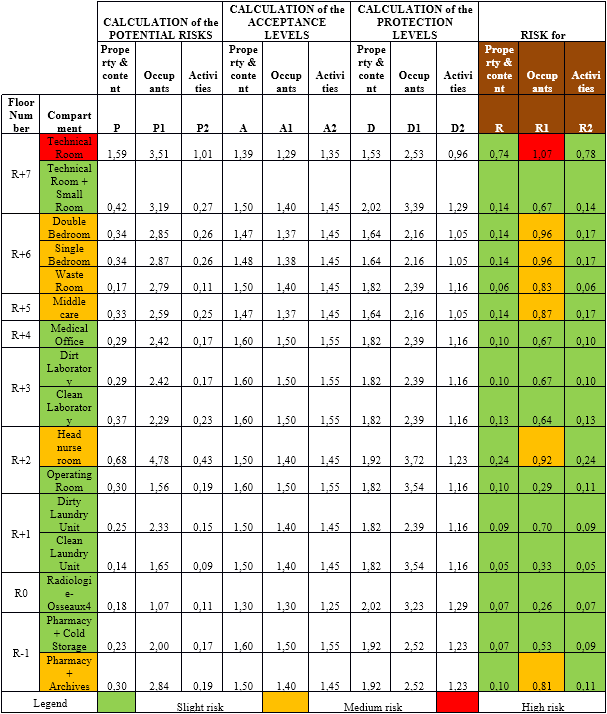
\includegraphics[keepaspectratio=true,width=\dimmin{}{\dimwidth{1.00}}]{images/TAB_FRAME}{}\mdline{446}%mdk

%mdk-data-line={447}
\mdhr{}%mdk

%mdk-data-line={448}
\noindent\mdline{448}\mdcaption{\textbf{Table~\mdcaptionlabel{6}.}~\mdcaptiontext{FRAME method results for the G Bloc of the Clinique Sainte Elisabeth}}%mdk
%mdk
\end{mdcenter}\label{tab-frame}%mdk
%mdk
\end{table}%mdk

%mdk-data-line={451}
\noindent\mdline{451}Since the 7th floor is not accessible to the public and the patients, the
most critical floor is the 6th floor in which people could be found
during the day and at night.%mdk

%mdk-data-line={455}
\subsection{\mdline{455}4.2.\hspace*{0.5em}\mdline{455}PATHFINDER RESULTS}\label{sec-pathfinder-results}%mdk%mdk

%mdk-data-line={457}
\noindent\mdline{457}The Pathfinder results have been categorized according to the different
scenarios simulated.%mdk

%mdk-data-line={460}
\subsubsection{\mdline{460}4.2.1.\hspace*{0.5em}\mdline{460}Scenario 1}\label{path-s1}%mdk%mdk

%mdk-data-line={462}
\noindent\mdline{462}The evacuation curve for the scenario 1 is shown in Figure\mdline{462}~\mdref{fig-evac-curve-s1}{\mdcaptionlabel{3}}\mdline{462}. The mean
total evacuation time of ambulant patients is about 383 seconds, with a
range of value between 163 seconds and 622 seconds.%mdk

%mdk-data-line={466}
\begin{figure}[tbp]%mdk
\begin{mdcenter}%mdk

%mdk-data-line={467}
\noindent\mdline{467}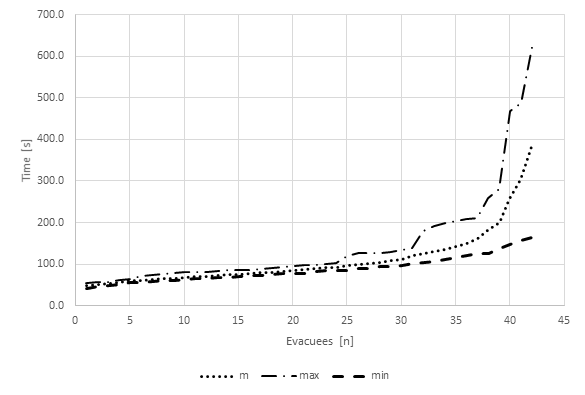
\includegraphics[keepaspectratio=true,width=\dimmin{}{\dimwidth{1.00}}]{images/evac-curve-scenario1}{}\mdline{467}%mdk

%mdk-data-line={468}
\mdhr{}%mdk

%mdk-data-line={469}
\noindent\mdline{469}\mdcaption{\textbf{Figure~\mdcaptionlabel{3}.}~\mdcaptiontext{Evacuation curve for scenario 1 (m is the mean evacuation curve, max is the maximum evacuation curve and min is the minimum evacuation curve)}}%mdk
%mdk
\end{mdcenter}\label{fig-evac-curve-s1}%mdk
%mdk
\end{figure}%mdk

%mdk-data-line={473}
\subsubsection{\mdline{473}4.2.2.\hspace*{0.5em}\mdline{473}Scenario 2}\label{path-s2}%mdk%mdk

%mdk-data-line={475}
\noindent\mdline{475}A comparison between the mean evacuation curves of scenarios 1 and 2
is shown in Figure\mdline{476}~\mdref{mean-evac-curve_s1-s2}{\mdcaptionlabel{4}}\mdline{476}. The results demonstrate that there is an
increase in total evacuation time when assisted evacuation is performed
involving dependent and highly-dependent patients. In fact, for
sub-scenario 2.1, in presence of 6 attendants to assist on the evacuation
of dependent patients, the evacuation of all the patients takes in
average about 483 seconds. For sub-scenario 2.2, in presence of 6
attendants to assist on the evacuation of dependent and highly-dependent
patients, the total evacuation takes in average about 2124 seconds.%mdk

%mdk-data-line={485}
\mdline{485}Comparing the mean total evacuation times of scenarios 1 and 2, one can
say that conducting an evacuation in presence of assisted patients
takes a higher time than a \mdline{487}\textquotedblleft{}normal\textquotedblright{}\mdline{487} evacuation (involving ambulant patients only). This is due to the fact
that the evacuation of dependent and highly-dependent patients is delayed
due to the preparation times required and the waiting for someone to assist them before starting to evacuate.
Furthermore, when considering only dependent patients, there is a slight increase of the total evacuation time, while when considering a mix of dependent and highly-dependent patients, the increase of total evacuation time is extremely higher. This is due to the fact that (1) the time required to prepare highly-dependent patients is higher than the time required to prepare dependent patients and, (2) when evacuating a highly-dependent patient, the group (nurses\mdline{490} \mdline{490}+ the patient) evolves at a reduced velocity comparing to the case when they assist on the evacuation of a dependent patient.%mdk

%mdk-data-line={492}
\begin{figure}[tbp]%mdk
\begin{mdcenter}%mdk

%mdk-data-line={493}
\noindent\mdline{493}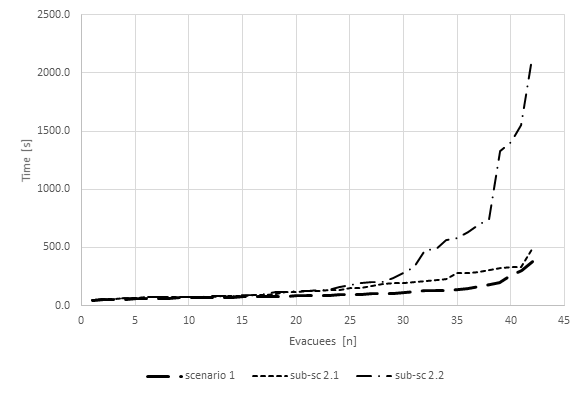
\includegraphics[keepaspectratio=true,width=\dimmin{}{\dimwidth{1.00}}]{images/mean-evac-curve-s1_s2}{}\mdline{493}%mdk

%mdk-data-line={494}
\mdhr{}%mdk

%mdk-data-line={495}
\noindent\mdline{495}\mdcaption{\textbf{Figure~\mdcaptionlabel{4}.}~\mdcaptiontext{Comparison of the mean evacuation curves for scenario 1 and 2}}%mdk
%mdk
\end{mdcenter}\label{mean-evac-curve_s1-s2}%mdk
%mdk
\end{figure}%mdk

%mdk-data-line={498}
\subsubsection{\mdline{498}4.2.3.\hspace*{0.5em}\mdline{498}Scenario 3}\label{path-s3}%mdk%mdk

%mdk-data-line={499}
\noindent\mdline{499}The results from the scenario 3, compared in Figure\mdline{499}~\mdref{fig-evac-curve-s3}{\mdcaptionlabel{5}}\mdline{499}, show that there is an 
increase in total evacuation time when considering a lower number of 
attendants. Indeed, when considering 6 EG (12 attendants) the total 
evacuation time is about 35 minutes, while when only 4 EG (8 attendants) 
are present, the total evacuation time increase to about 48 minutes. 
If we continue to reduce the number of emergency groups (e.g. evacuation
 during the night), a safe evacuation of the non-ambulant patients will 
 not necessarily be guaranteed, since the total evacuation times will reach
  extremely high values.%mdk

%mdk-data-line={510}
\begin{figure}[tbp]%mdk
\begin{mdcenter}%mdk

%mdk-data-line={511}
\noindent\mdline{511}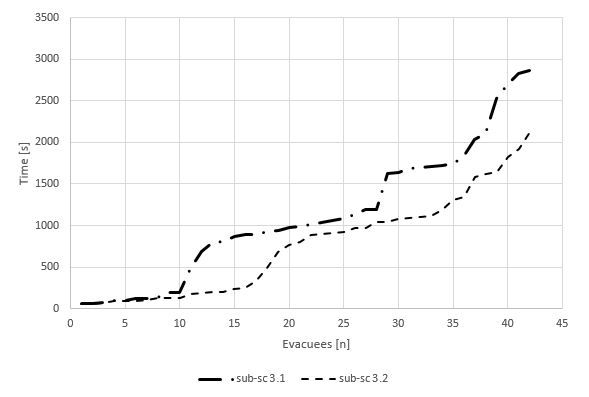
\includegraphics[keepaspectratio=true,width=\dimmin{}{\dimwidth{1.00}}]{images/evac-curve-scenario3}{}\mdline{511}%mdk

%mdk-data-line={512}
\mdhr{}%mdk

%mdk-data-line={513}
\noindent\mdline{513}\mdcaption{\textbf{Figure~\mdcaptionlabel{5}.}~\mdcaptiontext{comparison of evacuation curves for scenario 3 }}%mdk
%mdk
\end{mdcenter}\label{fig-evac-curve-s3}%mdk
%mdk
\end{figure}%mdk

%mdk-data-line={518}
\section{\mdline{518}5.\hspace*{0.5em}\mdline{518}CONCLUSIONS}\label{sec-conclusions}%mdk%mdk

%mdk-data-line={519}
\noindent\mdline{519}The main objectives of this paper were: (1) the simulation of prescript 
assisted evacuation using and agent based model, i.e. Pathfinder2016; 
(2) the evaluation of the effect of different numbers and categories 
of people with reduced mobility on the evacuation process; and, (3) 
the study of the impact of staff to patient’s ratio on the evacuation 
process.%mdk

%mdk-data-line={526}
\mdline{526}The analysis of the results showed that (1) conducting an assisted evacuation
 takes a higher time than an evacuation involving ambulant patients only (2) 
 the number of non-ambulant patients in the event of a fire should be designed 
 to be as few as possible. This may be achieved by establishing a number of 
 protected areas within the floors. Restricting the number of patients within
  each protected area will be of benefit in an evacuation in terms of fewer 
  patients requiring to be moved away from the fire and reducing the total
   evacuation time needed; (3) the type of non-ambulant patients involved
    on the evacuation process influence the total evacuation time. Indeed, 
    evacuating highly-dependent patients lead to a higher total evacuation 
    time than evacuating dependent patients; and, (4) the presence of a
     large number of attendants leads to faster evacuation.%mdk

%mdk-data-line={539}
\section{\mdline{539}6.\hspace*{0.5em}\mdline{539}FUTURE WORK}\label{sec-future-work}%mdk%mdk

%mdk-data-line={541}
\noindent\mdline{541}This research highlighted a lack of data about preparation times, the
number of attendants needed to assist the non-ambulant patients during
the evacuation process and the walking speeds. Future data collection
efforts are required to collect and analyze these variables.%mdk

%mdk-data-line={546}
\mdline{546}Further to this, more research is required to evaluate the effect of
stress and fatigue perceived by the attendants during the patient\mdline{547}'\mdline{547}s
collection.%mdk

%mdk-data-line={550}
\mdline{550}In addition, future works could investigate the impact of training of the
attendants on the evacuation time. Virtual Reality gaming could be used
in the future to provide valuable insight into a real life simulation and
highlight areas of risk.%mdk

%mdk-data-line={555}
\mdline{555}Finally, future research could focus on the coupling of this analysis
with the study of the possible effect of the fire itself. In fact, the
fire has a direct effect on the evacuating population, e.g., the presence
of the fire and smoke affects the people behavior, and there would be
the need to simulate this impact on the evacuation process.%mdk

%mdk-data-line={561;out/document-bib.bbl.mdk:1}
%mdk-data-line={561;out/document-bib.bbl.mdk:2}
\mdsetrefname{REFERENCES}%mdk
{\mdbibindent{0}%mdk
\begin{thebibliography}{36}%mdk
\label{sec-bibliography}%mdk

%mdk-data-line={references.bib:20}
\bibitem{3}Santos; B.E.~Aguirre. \textquotedblleft{}A Critical Review of Emergency Evacuation Simulation Models.\textquotedblright{} In \emph{Proceeding of the NIST Workshop on Building Occupant Movement during Fire Emergencies}, 25–50. NIST, Gaithersburg, USA.~Oct. 6AD.\label{3}%mdk%mdk

%mdk-data-line={references.bib:147}
\bibitem{18}Alonso. \emph{Egress Modelling in Health Care Occupancies}. The Fire Protection Research Foundation, Technical Notes, USA.~7AD.\label{18}%mdk%mdk

%mdk-data-line={references.bib:109}
\bibitem{13}Cuesta; O.~Abreu; D.~Alvear. \textquotedblleft{}Evacuation Modeling Trends.\textquotedblright{} Springer. 2016.\label{13}%mdk%mdk

%mdk-data-line={references.bib:31}
\bibitem{4}J.E Castle. \emph{Guidelines for Assessing Pedestrian Evacuation Software Applications}. Edited by Centre for Advanced Spatial Analysis. University College London, London. 2007.\label{4}%mdk%mdk

%mdk-data-line={references.bib:66}
\bibitem{8}Yuya Christensen Keith; Sasaki. \textquotedblleft{}Agent-Based Emergency Evacuation Simulation with Individuals with Disabilities in the Population.\textquotedblright{} \emph{Journal of Artificial Societies and Social Simulation} 11 (3): 9. 2008. \href{http://jasss.soc.surrey.ac.uk/11/3/9.html}{{\ttfamily http://\hspace{0pt}jasss.\hspace{0pt}soc.\hspace{0pt}surrey.\hspace{0pt}ac.\hspace{0pt}uk/\hspace{0pt}11/\hspace{0pt}3/\hspace{0pt}9.\hspace{0pt}html}}.\label{8}%mdk%mdk

%mdk-data-line={references.bib:260}
\bibitem{31}Rahouti; S.~Datoussaïd. \textquotedblleft{}Prédiction Du Risque Incendie En Milieu Hospitalier.\textquotedblright{} In \emph{GISEH16:La 8ème Conférence Francophone En Gestion et Ingénierie Des Systèmes Hospitaliers}. 2016.\label{31}%mdk%mdk

%mdk-data-line={references.bib:40}
\bibitem{5}M.V Gwynne; E.R.~Galea; M.~Owen; P.J.~Lawrence; L.~Fillipidis. \textquotedblleft{}Review of Modelling Methodologies Used in the Simulation of Evacuation.\textquotedblright{} \emph{J.~Build. Environ., 34}. 1999.\label{5}%mdk%mdk

%mdk-data-line={references.bib:247}
\bibitem{29}Project FiRE-TECH.~\textquotedblleft{}Fire Risk Evaluation to European Cultural Heritage European Study into the Fire Risk to European Cultural Heritage:WG6: Fire Risk Assessment Methods Draft Final Report.\textquotedblright{} \href{http://www.framemethod.net/indexen_html_files/wg6finalreport.pdf}{{\ttfamily http://\hspace{0pt}www.\hspace{0pt}framemethod.\hspace{0pt}net/\hspace{0pt}indexen\_\hspace{0pt}html\_\hspace{0pt}files/\hspace{0pt}wg6finalreport.\hspace{0pt}pdf}}.\label{29}%mdk%mdk

%mdk-data-line={references.bib:191}
\bibitem{22}John J Fruin. \emph{Pedestrian Planning and Design}. Book; Book/Illustrated. Revised ed. Mobile, AL : Elevator World. 1987. Based on the author’s thesis, originally presented at the Polytechnic Institute of Brooklyn under the title: Designing for pedestrians.\label{22}%mdk%mdk

%mdk-data-line={references.bib:165}
\bibitem{20}P.M.~Adams; E.R.~Galea. \textquotedblleft{}An Experimental Evaluation of Movement Devices Used to Assist People with Reduced Mobility in High-Rise Building Evacuations.\textquotedblright{} In \emph{Pedestrian and Evacuation Dynamics 2010, 5th International Conference}, edited by E.D.; Averill, J.D.~Peacock R.D.; Kuligowski, 129–138. Springer, New York, NY.~3AD.\label{20}%mdk%mdk

%mdk-data-line={references.bib:312}
\bibitem{37}Walts; J.~Stanford; P.~Weydeck; J.~Lukat; C.~Larsen; G.~Benigni; C.~Grady; C.~Gallaher. \emph{Hospital Evacuation Toolkit}. Florida Department of Health. 2011.\label{37}%mdk%mdk

%mdk-data-line={references.bib:130}
\bibitem{16}STEPS - Simulation Group. \emph{STEPS (Simulation of Transient Evacuation and Pedestrian Movements) User Manual}. Edited by Mott MacDonald. Croydon, UK.~2011.\label{16}%mdk%mdk

%mdk-data-line={references.bib:294}
\bibitem{35}Gwynne; E.R.~Galea; J.~Parke; J Hickson. \textquotedblleft{}The Collection of Pre-Evacuation Times from Evacuation Trials Involving Hospital Outpatient Facility, in Evans DD.\textquotedblright{} In \emph{Proceedings of the 7th International Symposium Fire Safety Science}, 877–888. IAFSS.~2002.\label{35}%mdk%mdk

%mdk-data-line={references.bib:284}
\bibitem{34}Gwynne; E.R.~Galea; J.~Parke; J Hickson. \textquotedblleft{}The Collection and Analysis of Pre-Evacuation Time Data Collected from Evacuation Trials and Their Application to Evacuation Modeling.\textquotedblright{} \emph{Fire Technology}, number 2,39: 179–195. 2003.\label{34}%mdk%mdk

%mdk-data-line={references.bib:3}
\bibitem{2}D.~Kuligowski; R.D.~Peacock; B.L.~Hoskins. \emph{Technical Note 1680:A Review of Building Evacuation Models (2nd Edition)}. Techreport. NIST, Gaithersburg, USA.~2010.\label{2}%mdk%mdk

%mdk-data-line={references.bib:267}
\bibitem{32}T.~Korhonen; S.~Hostikka. \emph{Fire Dynamics Simulator with Evacuation – FDS+Evac, Version 2.5.0 – Technical Reference and User’s Guide}. VTT, Helsinki, Finland. 2009.\label{32}%mdk%mdk

%mdk-data-line={references.bib:86}
\bibitem{10}A.~Hunt. \textquotedblleft{}Simulating Hospital Evacuation.\textquotedblright{} Phdthesis, University of Greenwich. 2016.\label{10}%mdk%mdk

%mdk-data-line={references.bib:93}
\bibitem{11}W.~Johnson. \emph{Using Computer Simulations to Support a Risk-Based Approach for Hospital Evacuation}. Glasgow Accident Analysis Group, Department of Computing Science, University of Glasgow, Glasgow, UK.~2006.\label{11}%mdk%mdk

%mdk-data-line={references.bib:48}
\bibitem{6}M.V Gwynne; D.~Kuligowski. \textquotedblleft{}Application Modes of Egress Simulation.\textquotedblright{} In \emph{Proceeding of Pedestrian and Evacuation Dynamics}, 397–409. Wuppertal, Germany. 2008.\label{6}%mdk%mdk

%mdk-data-line={references.bib:176}
\bibitem{21}A.~Hunt; E.R.~Galea; P.~Lawrence. \textquotedblleft{}An Analysis and Numerical Simulation of the Performance of Trained Hospital Staff Using Movement Assist Devices to Evacuate People with Reduced Mobility.\textquotedblright{} \emph{Fire and Materials} 39 (4). Wiley-Blackwell: 407–429. Dec. 2013. doi:\href{https://dx.doi.org/10.1002/fam.2215}{10.1002/fam.2215}.\label{21}%mdk%mdk

%mdk-data-line={references.bib:78}
\bibitem{9}Parke; S.~Gwynne; E.~Galea; P.~Lawrence. \textquotedblleft{}Validating the buildingEXODUS Evacuation Model Using Data from an Unannounced Trial Evacuation.\textquotedblright{} In \emph{Proceedings of 2nd International Pedestrian and Evacuation Dynamics Conference}. London, UK.~2003.\label{9}%mdk%mdk

%mdk-data-line={references.bib:57}
\bibitem{7}M.~Levin. \textquotedblleft{}EXITT- A Simulation Model of Occupant Decisions and Actions in Residential Fires.\textquotedblright{} In \emph{Proceedings of the 2nd International Symposium on Fire Safety Science}. Tokyo, Japan. 1989.\label{7}%mdk%mdk

%mdk-data-line={references.bib:122}
\bibitem{15}T.~Korhonen; S.~Hostikka; Heliövaara; H.~S Ehtamo; K.~Matikainen. \textquotedblleft{}FDS+Evac: Evacuation Module for Fire Dynamics Simulator.\textquotedblright{} In \emph{Interflam2007: 11th International Conference on Fire Science and Engineering}. London, UK.~2007.\label{15}%mdk%mdk

%mdk-data-line={references.bib:275}
\bibitem{33}Nelson, and F.~Mowrer. \textquotedblleft{}Emergency Movement.\textquotedblright{} In \emph{SFPE Handbook of Fire Protection Engineering, Third Ed.}, edited by P.~DiNenno. Quincy, MA.~2002.\label{33}%mdk%mdk

%mdk-data-line={references.bib:204}
\bibitem{23}International Maritime Organization, editor. \emph{MSC Circ. 1248, Interim Guidelines for Evacuation Analyses for New and Existing Passenger Ships}. 2002.\label{23}%mdk%mdk

%mdk-data-line={references.bib:156}
\bibitem{19}Ursetta; A.~D’Orazio; L.~Grossi; G.~Carbotti; S.~Casentini; L.~Poggi. \emph{Egress from a Hospital Ward: A Case Study}. FEMTC2014: Fire and Evacuation Modeling Technical Conference 2014. 2014. \href{http://www.thunderheadeng.com/2014/10/femtc2014_d2-b-3_carbotti/}{{\ttfamily http://\hspace{0pt}www.\hspace{0pt}thunderheadeng.\hspace{0pt}com/\hspace{0pt}2014/\hspace{0pt}10/\hspace{0pt}femtc2014\_\hspace{0pt}d2-\hspace{0pt}b-\hspace{0pt}3\_\hspace{0pt}carbotti/\hspace{0pt}}}.\label{19}%mdk%mdk

%mdk-data-line={references.bib:13}
\bibitem{1}Centre fédéral de connaissances pour la civile Sécurité. \emph{Statistiques 2013 Des Services D’incendie Belges}. Techreport. 2013.\label{1}%mdk%mdk

%mdk-data-line={references.bib:138}
\bibitem{17}Golmohamamdi; D.~Shimshak. \textquotedblleft{}Estimation of the Evacuation Time in an Emergency Situation in Hospitals.\textquotedblright{} \emph{Computer and Industrial Engineering}, 1256–1267. 2001.\label{17}%mdk%mdk

%mdk-data-line={references.bib:303}
\bibitem{36}E.~Boyce; T.J.~Shields; G.W.H.~Silcock. \textquotedblleft{}Toward the Characterization of Building Occupancies for Fire Safety Engineering: Capabilities of Disabled People Moving Horizontally and on an Incline.\textquotedblright{} \emph{Fire Technology}, number 35: 51–67. 1999.\label{36}%mdk%mdk

%mdk-data-line={references.bib:219}
\bibitem{25}De Smet. \textquotedblleft{}F.R.A.M.E: Fire Risk Assessment Method for Engineering.\textquotedblright{} Sep. 2016. Accessed September 19. \href{http://www.framemethod.net/indexen.html}{{\ttfamily http://\hspace{0pt}www.\hspace{0pt}framemethod.\hspace{0pt}net/\hspace{0pt}indexen.\hspace{0pt}html}}.\label{25}%mdk%mdk

%mdk-data-line={references.bib:226}
\bibitem{26}De Smet. \textquotedblleft{}F.R.A.M.E Calculation Report: Düsseldorf Airport.\textquotedblright{} Sep. 2016. Accessed September 19. \href{http://www.framemethod.net/indexen_15.html}{{\ttfamily http://\hspace{0pt}www.\hspace{0pt}framemethod.\hspace{0pt}net/\hspace{0pt}indexen\_\hspace{0pt}15.\hspace{0pt}html}}.\label{26}%mdk%mdk

%mdk-data-line={references.bib:233}
\bibitem{27}De Smet. \textquotedblleft{}F.R.A.M.E Calculation Report: Sofa Super Store Fire.\textquotedblright{} Sep. 2016. Accessed September 19. \href{http://www.framemethod.net/indexen_23.html}{{\ttfamily http://\hspace{0pt}www.\hspace{0pt}framemethod.\hspace{0pt}net/\hspace{0pt}indexen\_\hspace{0pt}23.\hspace{0pt}html}}.\label{27}%mdk%mdk

%mdk-data-line={references.bib:240}
\bibitem{28}De Smet. \textquotedblleft{}Example: Historic Building: 13-15 Century Monastery Used as Museum and Cultural Centre.\textquotedblright{} Sep. 2016. Accessed September 19. \href{http://www.framemethod.net/indexen_20.html}{{\ttfamily http://\hspace{0pt}www.\hspace{0pt}framemethod.\hspace{0pt}net/\hspace{0pt}indexen\_\hspace{0pt}20.\hspace{0pt}html}}.\label{28}%mdk%mdk

%mdk-data-line={references.bib:254}
\bibitem{30}De Smet. \textquotedblleft{}F.R.A.M.E Calculation Report: Kanunnick Triest Te Melle.\textquotedblright{} \href{http://www.framemethod.net/indexnl_html_files/Brand\%2520in\%2520Zorgcentrum\%2520Kanunnik\%2520Triest\%2520te\%2520Melle.pdf}{{\ttfamily http://\hspace{0pt}www.\hspace{0pt}framemethod.\hspace{0pt}net/\hspace{0pt}indexnl\_\hspace{0pt}html\_\hspace{0pt}files/\hspace{0pt}Brand\hspace{0pt}\%20in\hspace{0pt}\%20Zorgcentrum\hspace{0pt}\%20Kanunnik\hspace{0pt}\%20Triest\hspace{0pt}\%20te\hspace{0pt}\%20Melle.\hspace{0pt}pdf}}.\label{30}%mdk%mdk

%mdk-data-line={references.bib:116}
\bibitem{14}Thunderhead. \emph{Pathfinder 2016, Technical Reference}. 2016.\label{14}%mdk%mdk

%mdk-data-line={references.bib:101}
\bibitem{12}Uehara; K.~Tomomatsu. \textquotedblleft{}Evacuation Simulation System Considering Evacuee Profiles and Spatial Characteristics.\textquotedblright{} In \emph{Proceedings of the 7th International Symposium of Safety Science}, 963–974. 2001.\label{12}%mdk%mdk
\par%mdk
\end{thebibliography}}%mdk%mdk%mdk


\end{document}
